\section{Sprint planning}
\subsection{User-stories}
\subsubsection*{Implementation}
All the functional requirements for sprint 5 are presented in table \ref{tab:sprint5stories}
\LTXtable{\textwidth}{sprint5/stories.tex}

\subsubsection*{Documentation}
All the documentation stories for sprint 5 are presented in table \ref{tab:sprint5Documentationstories}
\LTXtable{\textwidth}{sprint5/storiesDocumentation.tex}

\subsubsection*{Project management}
All the project management for sprint 5 are presented in table \ref{tab:sprint5storiesProcess}
\LTXtable{\textwidth}{sprint5/storiesProcess.tex}

% hous all in total: Estimated: 235  Spent: 230
\section{System Burndown}

\begin{figure}[H]
	\centering
		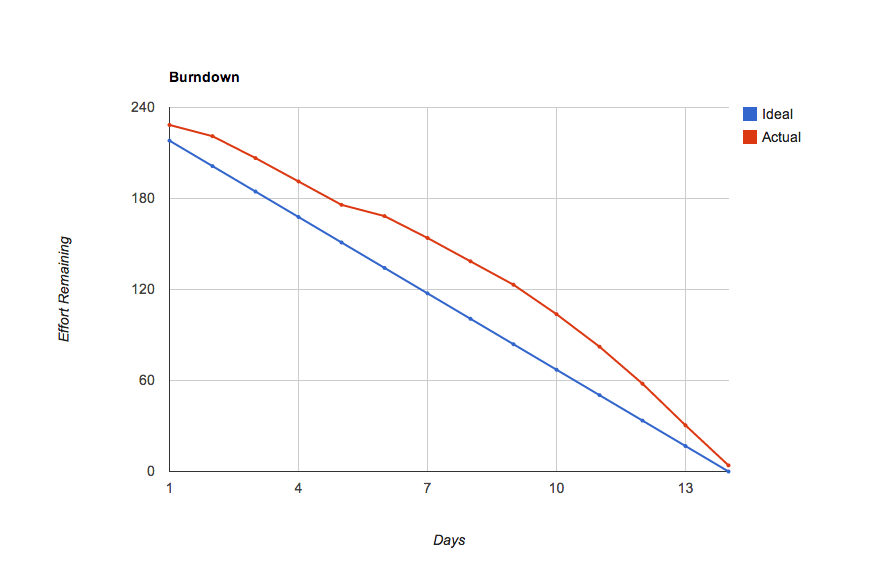
\includegraphics[width=18cm]{sprint5/BurndownSprint5.png}
	\caption{Burn down chart.}
	\label{fig:Burn5 }
\end{figure}

\section{Architecture}
\begin{figure}[H]
	\centering
		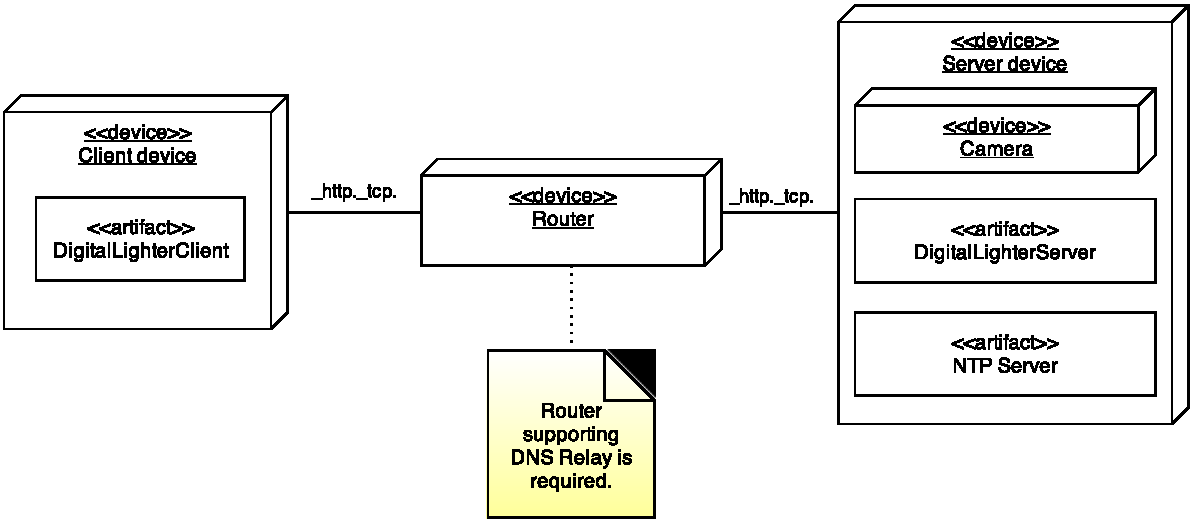
\includegraphics[width=15cm]{images/deployment-diagram-sprint5}
	\caption{Deployment diagram}
	\label{fig:sprint5_deployment_diagram}
\end{figure}
\section{Implementation}
\section{Testing}
\section{Occurring risks}
\section{Customer feedback}
\section{Retrospective}
This section reflects on the past sprint. In order to learn from the mistakes done and thus to improve the workflow it is necessary to answer two essential questions: "What went well" and "What could be improved".

\subsection{What went well}
\subsection{What could be improved}
